% Many thanks to Andrew West for writing most of this file
% Main LaTeX file for CIS400/401 Project Proposal Specification
%
% Once built and in PDF form this document outlines the format of a
% project proposal. However, in raw (.tex) form, we also try to
% comment on some basic LaTeX technique. This is not intended to be a
% LaTeX tutorial, instead just (1) a use-case thereof, and (2) a
% template for your own writing.

% Ordinarily we'd begin by specifying some broad document properties
% like font-size, page-size, margins, etc. -- We have done this (and
% much more) for you by creating a 'style file', which the
% 'documentclass' command references.
\documentclass{sig-alternate}

% These 'usepackage' commands are a way of importing additional LaTeX
% styles and formattings that aren't part of the 'standard library'
\usepackage{mdwlist}
\usepackage{url}
\usepackage{graphics}

\begin{document}

% We setup the parameters to our title header before 'making' it. Note
% that your proposals should have actual titles, not the generic one
% we have here.
\title{Platform for Evaluating Real-Time Resource Management Algorithms for Network Function Virtualization}
\subtitle{Dept. of CIS - Senior Design 2014-2015\thanks{Advisor: Linh Thi Xuan Phan (linhphan@cis.upenn.edu).}}
\author{
\alignauthor Alex Brashear, Razzi Abuissa, Dong Young Kim, Alex Lyons\\
\vspace{.4cm}
University of Pennsylvania\\
Philadelphia, PA \\
\vspace{.4cm}
\texttt{\{brashear, rabuissa, kido, allyons\}@seas.upenn.edu}
}

\date{}
\maketitle

% Next we write out our abstract -- generally a two paragraph maximum,
% executive summary of the motivation and contributions of the work.
\begin{abstract}
 \textit{Network Functions Virtualization (NFV) is an approach to implementing network infrastructure that emerged in 2012. NFV aims to address the inflexibility of classical network hardware by leveraging virtualization technology to consolidate network equipment onto industry standard servers. To date, several reports have demonstrated the feasibility of virtualizing network functions. (cite) In order for NFV to succeed in practice, it is desirable for virtualized network systems to be able to meet real-time deadlines. To that end, Professor Linh Phan and her research group at Penn have developed algorithms to manage computing and network resources to implement virtualized network functions given real-time constraints.}

 \textit{One application of real-time NFV is to provide network services that meet end-to-end latency requirements. In this project, we propose to design and implement a testing platform that simulates a service provider that, given an algorithm for research management, provides services meeting real-time constraints. In doing so, the platform can evaluate the effectiveness of the resource management algorithm. We will perform trials to collect metrics to analyze and eventually improve the real-time scheduling algorithms. The testing platform will consist of an orchestration layer and a cluster of computers that provide computing and networking resources. This system will enable the evaluation of the algorithms and aid in the development of future algorithms for implementing network functions subject to time constraints.}
\end{abstract}

\begin{figure*}[htb!]
 \begin{center}
   \includegraphics[width=16cm]{service_provider}
 \end{center}
 \vspace{-12pt}
 \caption{A block-flow diagram of the core components of the service provider}
 \label{fig:some_graph}
\end{figure*}

% Then we proceed into the body of the report itself. The effect of
% the 'section' command is obvious, but also notice 'label'. Its good
% practice to label every (sub)-section, graph, equation etc. -- this
% gives us a way to dynamically reference it later in the text via the
% 'ref' command, e.g., instead of writing `Section 1', you can write
% `Section~\ref{sec:intro}', which is useful if the section number
% changes.
\section{Introduction}
\label{sec:intro}
A variety of network appliances provide important services by mediating data packets sent on the network. Such appliances filter or manipulate packets in order to improve the efficiency and security of the network. A firewall is an example of a middlebox that filters out malicious or irrelevant traffic. However, network hardware poses a growing problem because it is difficult to install and maintain. Furthermore, middleboxes burden enterprises with financial and administrative cost \cite{white_paper}. In the same way that cloud computing freed service providers from the management of physical hardware, Network Functions Virtualization (NFV) has been proposed as a solution to move network hardware functions to the cloud, where hardware services can be managed by software. NFV can make it easier for network administrators to install, manage, and upgrade networking devices \cite{white_paper}.

Suppose a service provider wants to virtualize hardware network functions in order to benefit from NFV in terms of economic savings, automation, and scalability. One desirable feature such a service provider could offer is the guarantee that customer data will be processed and returned within an acceptable time frame. The service provider then has the challenge of managing its resources to meet this criteria. Although research has shown that it can be beneficial to move network hardware to the cloud, few studies have been conducted to suggest ways to manage resources for network functions in such a way that they meet real-time constraints.

Recently, Dr. Phan and her research gropu at the University of Pennsylvania has developed an algorithm that can schedule and manage NFV services in the cloud in order to meet real-time constraints, allowing services to be scheduled on virtual machines on demand. The algorithm's main goal is to create effective configuration of virtual machines in the cloud and schedule services in a way that minimizes latency in order the meet the latency requirement. At a high level, the algorithm uses a combination of linear programming and real time analysis to determine the assignment of services to virtual machines in the cloud. In middleboxes, a data packet coming from a customer will be processed by the first service, and then the output of that will be sent to the second service to be processed, then the third, and so on. When scheduling services in the cloud, it is optimal to place services within close proximity to one another in order to minimize the latency that will be incurred with the distance that packets have to travel from service to another, after being processed. Another important consideration that the algorithm looks at is effective ways to schedule CPU and network resources on the cloud. Both allocations of CPU and network resources occur in real time based on the latency requirement imposed by customers. The algorithm tries to ensure that the end-to-end latency, or the total latency acquired from processing a data packet through the chain of services from the virtual machines, is minimized.

Currently, no analysis platform exists to evaluate effective resource management algorithms for virtualized network functions on the cloud. As our research project, we propose a testing platform that can be used to analyze the ability of network service scheduling algorithms to meet customer latency requirements. Specifically, we propose to create software that simulate a service provider in the cloud handling customer requests. Through careful design of this software, it can be used to test and prove the correctness of real-time scheduling algorithms. On a broader standpoint, this software will ultimately help cloud service provider make real-time latency guarantees to customers. The specifics of this system is described below.
% The header of this document might have been a little intimidatating
% to beginners. Notice once you are in the body of the document,
% however, LaTeX commands are minimal and 'normal text' is frequent.


\section{Related Work}
\label{sec:related_work}
Although research into Network Functions Virtualization is a recent phenomenon, substantial progress in the field has led to numerous technological innovations. The following research examples serve as a collective proof-of-concept, demonstrating that, among other things, network functions can be virtualized and algorithms can be designed to minimize latency. Furthermore, they suggest that NFV is not only technologically feasible but economically viable as well.

A white paper published by the European Telecommunications Standards Institute defined Network Functions Virtualization and outlined the benefits and challenges associated \cite{white_paper}. This paper covers many practical aspects of NFV and is a key motivation for research in this area, and especially useful to our research because it clearly defines the goals of NFV in which we can use to evaluate our system and measure our progress.

Making Middleboxes Someone Else's Problem: Network Processing as a Cloud Service \cite{Sherry:2012:MMS:2342356.2342359} is one of the earliest practical studies of moving middlebox processing to the cloud. Like the white paper, this publication gives strong motivation for the field by surveying the current state of network enterprises. This research highlights several design choices of the system they implemented which successfully mitigates potential weaknesses of NFV. This study touches upon scaling middleboxes in response to load, but does so on a small scale and does not impose time constraints on the network functions.

One specific technology that is relevant to our research is ClickOS and the Art of Network Function Virtualization \cite{179771}, which deals specifically with high-performance virtualization of network functions. The strategies they used to optimize hypervisors and operating systems for network processing will be useful for building a performant system, and the fact that their patches to software such as Xen are open source means that we can use components of their work for high-performance NFV.

Design and Implementation of a Consolidated Middlebox Architecture \cite{Sekar:2012:DIC:2228298.2228331} will also be invaluable for reference because it deals specifically with deploying multiple virtualized middleboxes, which is exactly what we will be dealing with. The general techniques employed here will be useful, but they still do not impose time constraints and are more interested in aggregate statistics than specific reliability and performance quotas.

Additional research such as Theory of Scheduling and Routing \cite{DBLP:conf/fsttcs/BampisKLLS13} will help us understand the theoretical limits and state-of-the-art of scheduling.

This project, which will draw heavily upon the aforementioned research and technology as groundwork, gives unique consideration to performance guarantees in real-time systems. Current NFV resource-management algorithms seek to reduce average latency across all requests, but they cannot guarantee that a specific task will complete given a time constraint with minimal variance. This project establishes a platform for evaluating algorithms which seek compliance with various specific performance constraints.


\section{Project Proposal}
\label{sec:project_proposal}
Our group will develop software to configure a cluster of computers to act as a network functions service provider. Real-time resource management algorithms can then be evaluated by using them to manage the provider's computing and networking resources and simulating customers interacting with the provider. By measuring the success rate of the service provider to handle traffic within latency constraints, we will be able to analyze and improve the algorithms.

\subsection{Anticipated Approach}
\label{subsec:approach}

The service provider that we will be building to test the algorithms will consist of two major components: an orchestration layer and the hardware that provides computing and networking resources. The orchestration layer consists of a state manager, request handler, algorithm solver, and analytics monitor. The hardware consists of high-volume servers which host virtual machines and network switches which allow the machines to send and receive data.

The state manager will keep track of the computing fleet in terms of the software configuration and activity on each computer. When changes need to be made to the fleet, the state manager will put them into effect by creating, modifying or destroying virtual machines.

The request handler will expose an API to handle requests for services that specify functionality and performance requirements of the services. Depending on the service provider's capacity and usage, requests for services can either be accepted or rejected.

The algorithm solver will solve for resource management strategies given the customer requirements and the state of the fleet. The algorithm used by the solver can be switched out to evaluate different resource management algorithms across separate trials. The algorithm solver communicates with the state manager to enact the strategies it produces.

The analytics component will track of how the system is performing over time and if it is meeting the requirements imposed by the customers. Once a trial has finished, this information will be used to generate a quantitative report of the resource management algorithms.

The hardware will be provided by Professor Phan's research group as four 32-core computers and network switches to connect them.

Trials will start with orchestration layer running and only the base hypervisor installed on the computing hardware. Simulated customers will begin to make requests with information about the desired services, the acceptable latency (e.g. 20 ms), and the amount of data they will send (e.g. 100 mb at 1 mb / second). The request handler will accept or reject the requests. Once a request has been accepted, the customer will begin sending data to be processed and performance analytics will be collected by the service provider. When a trial is over, a report of the algorithm's performance over that trial will be generated.

\begin{figure}[htb!]
 \begin{flushleft}
   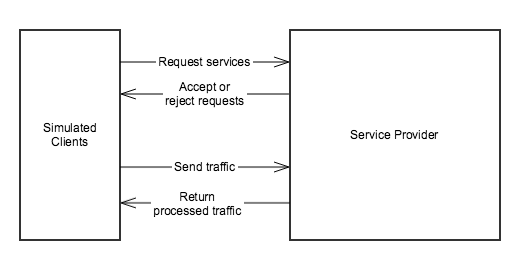
\includegraphics[width=9cm]{system}
 \end{flushleft}
 \vspace{-12pt}
 \caption{A high level illustration of interaction client between service provider}
 \label{fig:some_graph}
\end{figure}

\subsection{Technical Challenges}
\label{subsec:tech_challenges}

The nature of Network Function Virtualization requires the integration of complex hardware and software. This design complicates latency constraint handling because CPU resources and network resources must be managed simultaneously. A major design challenge in lieu of meeting real-time end-to-end latency guarantees is optimizing and measuring both processor- and network-sourced latencies. In order to achieve minimal end-to-end latency, our design will need to a) minimize the overhead of critical functions, and b) keep non-critical functions off of the critical path.

A related design challenge is achieving repeatable test results so that algorithms may be analyzed and compared to one another. In order to accomplish this, the system must also provide consistent latency. Our design also presents additional challenges including maintaining overall system reliability and recovering from the failure of individual components.

Finally, in order to provide a useful evaluation of the algorithm, the entire system has to be realistic. The service provider should consistently handle customer requests and traffic without mistakes. The trials should involve a variety of scenarios that will allow for the understanding of all facets of the resource management algorithm.

\subsection{Evaluation Criteria}
\label{subsec:eval_criteria}

We consider several evaluation metrics. First, we will use output from the analytics component of the platform to understand and validate the performance of the real-time scheduling algorithm. Specifically, we compare end-to-end latency produced from the chain of services scheduled in multicore computers against the algorithm's predicted latency. We plan to set an appropriate significance level in order to set a benchmark for acceptable latency performance. Since the algorithm schedules services in real-time based on the service's functional requirements (in latency), we will validate how the algorithm performs given a wide range of functional requirements.

Second, when building this platform, it is important to consider how much overhead our system adds to the providing services. If our system's design plays a significant factor in increasing end-to-end latency, then the software and design of our platform must be optimized to minimize unnecessary and significant overhead. In the next few weeks of designing our platform, we plan to define an acceptable measure of overhead. One obvious constraint to this measure is that the added overhead should not increase the end-to-end latency of the services to more than the latency requirement imposed by clients.

Lastly, we evaluate our platform based on its scalability. As mentioned above, we plan on building this testing platform on 4 multi-core computers that will simulate servers. When talking about the scalability of this system, we need to ensure that the system is able to steadily and efficiently handle large incoming traffic (substantial packets/second) as well as deal with strict functional requirements on the system.


\section{Research Timeline}
\label{sec:research_timeline}

As there is already a research group working on this subject, we will spend the first few weeks understanding the progress that has already been made by the group. Since this project involves a good deal of development, we will also spend this time on determining a set of frameworks and tools for the project. Since tools such as RT-Xen have already been used by the research group, it will be up to our senior design group to gain familiarity of these tools. This background work should be mostly completed by Thanksgiving break.

By Winter break, we will specify all the components and begin developing and testing each. We will also begin connecting components in an environment such as AWS EC2. Although performance metrics are unreliable as we are not in full control of the environment, this will allow us to make sure things are working as smoothly as possible.

Early in the spring semester, we will begin installing the components on the physical machines and begin collecting preliminary benchmarks. We will collect our first metrics by February and identify bottlenecks and architectural issues.

The rest of the year will be spent iterating on the system and performing trials with different resource management algorithms and analyzing the results. By this point we should have enough understanding of the algorithms that we can propose improvements to resource management.

As time permits, we will build an analytics dashboard for monitoring performance in real time for further insight, and contribute back to the open source tools that we used during our research.

% We next move onto the bibliography.
\bibliographystyle{plain} % Please do not change the bib-style
\bibliography{prop_spec}  % Just the *.BIB filename

% Here is a dirty hack. We insert so much vertical space that the
% appendices, which want to begin in the left colunm underneath
% "references", are pushed over to the right-hand column. If we looked
% hard enough, there is probably a command to do exactly this (and
% wouldn't need tweaked after edits).
% \vspace{175pt}

% We then use appendices to share some additional information with
% you, though you won't need appendices in your own proposal.


% This paragraph makes use of dynamic references. Remember how we've
% been 'label'-ing everything; sections, etc? Using 'ref' we can
% reference them. Add a new figure/section at the beginning? This
% technique automatically re-numbers when you build, so you don't have
% to make static changes.
% At this point, the proposal specification is complete. From here on
% out, we are just going to show off some commonly used \LaTeX{}
% technique. Be sure to look at the `code behind' and see
% Tab.~\ref{tab:some_table}, Eqn.~\ref{eqn:some_equation} and
% Fig.~\ref{fig:some_graph} for the output! Keep in mind that the
% appendix is usually not a good place for your figures. Place them
% where you need them and remember to refer to them in the body of your
% text; otherwise, the reader will keep reading and will miss them!

% We next encounter tables and figures (images). Big things like these
% are known as 'floats' in LaTeX because their position is not
% fixed. Notice that '[htb!]' follows the start of each
% environment. We are telling LaTeX that we'd like to put the
% table/fig 'h' - HERE, precisely where it follows in the
% narrative. If LaTeX determines it doesn't look good here, 't' tells
% LaTeX we'd like it at the top of this column, and if that doesn't
% work, use 'b', the bottom of the column. Other options are
% available. LaTeX shifts floats around to ensure images don't end up
% on page/column boundaries, which would result in a waste of space
% for text.

% We insert a graph/figure into the document. This is a pretty
% straightforward process once you get the image into a file format
% that LaTeX plays nice with. Then we just scale it as
% a % of the column width.

\end{document}



